\documentclass{standalone}
\usepackage{standalone}

\begin{document}
\section{Data Collection}
In our approach, we first tried to collect users Facebook profile data through Facebook Graph API with features like count, group activity no. of pictures uploads, check-in, birthday, place live in, education, age etc. But due to data restriction in current API version we failed to collect users profile data with sufficient features. Then we turn back and change our data collection approach. We created a form a with features Sex, Age, Religion and his/her Facebook status and collected approximately 250 users data. Below figure is showing the ratio of Male Female, Religion, Age. We tried to equalize the ratio of male female and religion.

\begin{figure}[h]
				\centering
				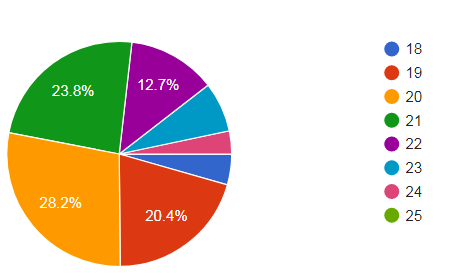
\includegraphics[scale=0.8]{./img/age}
				\caption{Users ratio according to Age} \label{fig:mapComp}
\end{figure}
\begin{figure}[h]
				\centering
				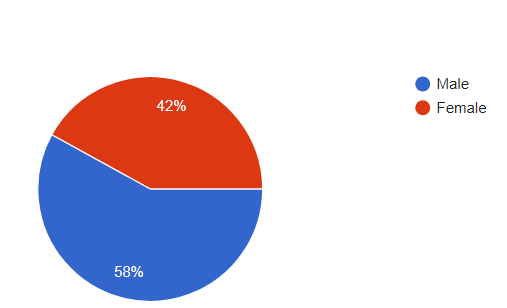
\includegraphics[scale=0.8]{./img/sex}
				\caption{Users ratio according to Sex} \label{fig:mapComp}
\end{figure}
\begin{figure}[h]
				\centering
				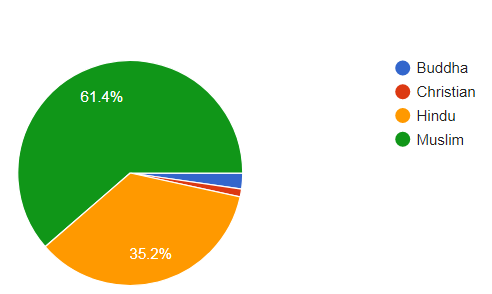
\includegraphics[scale=0.8]{./img/religion}
				\caption{Users ratio according to Religion} \label{fig:mapComp}
\end{figure}

\end{document}